\section{Имитационное моделирование}
В данной работе, для анализа полученных решений систем массового обслуживания с повторными вызовами и вызываемыми заявками используется имитационное моделирование. Построив имитационную модель системы, мы получаем возможность сравнить результаты ее работы с аналитическим решением для  оценки применимости полученных результатов путем сравнения численных характеристик.

Моделирование систем массового обслуживания сводится к генерированию случайных времен с соответствующим распределением вероятности, по прошествии которого в модели наступит некоторое событие - приход заявки, окончание обслуживания и т.д., что называется дискретно-событийным подходом. Таким образом, в течение моделирования на протяжении некоторого заданного времени модель генерирует и обрабатывает события системы, которые впоследствии регистрируются, и на их основе подсчитываются численные характеристики, такие как распределение вероятности.

Реализованная имитационная модель, как программный продукт, разрабатывалась с возможностью расширения ее функционала для предоставления возможности тонко настраивать параметры моделирования и без препятствий извлекать полученные результаты в виде распределения вероятности для последующего анализа. В этих целях, программа реализована при помощи объектно ориентированного подхода, так как данный подход позволил выстроить логику работу программы на уровне абстракций, что и дает возможность легкого расширения функционала и реализации моделей других систем массового обслуживания.

\subsection {Объектная модель предметной области}
Для построения объектной модели предметной области программы рассматриваются следующие объекты систем массового обслуживания, используемые в данной работе:
\begin{itemize}
\item Заявка - объект, который поступает в систему, перемещается по ней и , в конечном итоге, покидает систему в течение моделирования.
\item Обслуживающий прибор - объект, принимающий на вход заявки и обслуживающий их. По окончании обслуживания заявки покидают прибор.
\item Орбита - скопление заявок, ожидающих повторного обращения на обслуживающий прибор.
\item Входящий поток - объект, генерирующий заявки, которые поступают в систему.
	\end{itemize}
 Поскольку, процесс работы модели заключается в перемещении заявок по системе, то в некоторый момент времени моделирования $T_{mod}$ местонахождение каждой заявки и ее свойства могут меняться. В таком случае, необходимо отслуживать момент времени, в который заявка изменит свое состояние - $T_{del}$. В момент времени, когда $T_{del} = T_{mod}$,  происходит смена состояния заявки, и  $T_{del}$ обновляется объектом системы массового обслуживания, в которой она на данный момент находится. Среди событий , при которых происходит обновление момента смены состояния заявки, выделим следующие:
\begin{itemize}
	\item Заявка покидает входящий поток - в данном случае в источнике генерируется новая заявка с моментом времени $T_{del}$, при наступлении которого, она также покинет входящий поток.
	\item Заявка успешно поступила на прибор и начала обслуживаться - в этом случае обслуживающий прибор определяет для заявки момент времени $T_{del}$, в который ее обслуживание закончится.
	\item При попытке поступить на прибор заявка застала его занятым обслуживанием другой заявки и отправилась на орбиту. По прибытии на орбиту, новый момент времени $T_{del}$ заявки определяется как время, при наступлении которого заявка покинет орбиту.
\end{itemize}
Исходя из вышеописанного, центральными объектами в предметной области являются заявка и событие, наступающее в системе при смене состояния заявки. В предметной области они представлены классом Event, который связан ассоциацией с перечислением EventType, элементы которого соответствуют объектам системы обслуживания, в которых наступило  событие. Это позволяет собирать статистику о произошедших событиях в системе.
\begin{figure}[H]
	\centering
	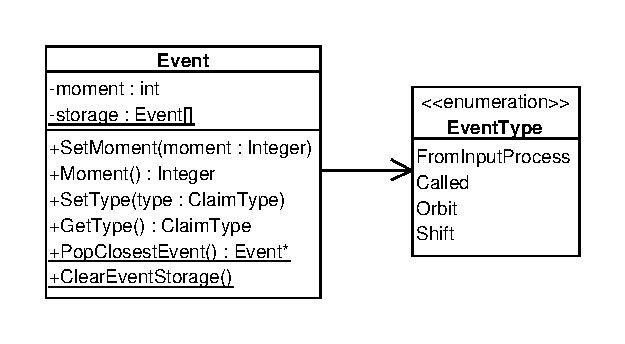
\includegraphics[scale=1]{event_uml.eps}
	\caption{Класс Event}
	\label{event_uml}
\end{figure}
Поле moment хранит момент времени $T_{del}$ до изменения состояния объекта. Для того, чтобы определить, какое событие должно произойти в модели следующим, класс Event содержит статическую коллекцию собственных объектов - storage. При создании новых событий они также помещаются и в storage для того, чтобы в последствии извлекать следующее по времени событие c помощью метода PopClosestEvent.

Для реализации подхода, основанном на постоянном обновлении состоянии заявок, находящихся в системе, предметная область базируется на общем интерфейсе, который реализуют все конкретные элементы рассматриваемых систем массового обслуживания. Его цель заключается в формализации изменения элемента  с каждым дискретным промежутком времени в течение моделирования. Поскольку, сам класс RQ-системы, как будет показано ниже, реализует данный интерфейс, то возможно использовать ее как входящий поток для другой системы.
\begin{figure}[H]
	\centering
	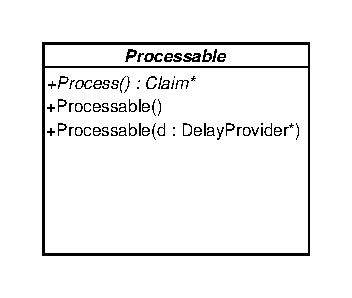
\includegraphics[scale=1]{processable_uml.eps}
	\caption{Общий интерфейс Processable для всех элементов системы массового обслуживания}
	\label{processable_uml}
\end{figure}
Метод Process унифицирует все изменения в элементе системы массового обслуживания, которые должны произойти в нем при наступлении события. Реализация этого интерфейса не обязательно должна иметь только этот метод, так как для удобства организации логики работы, удобно размещать некоторые алгоритмы в отдельным методах.

Также, не все элементы системы можно полностью описать данным интерфейсом - обслуживающий прибор и орбита, помимо общего метода Process, должны иметь и точки входа для заявок. По этой причине для них определены соответствующие интерфейсы, наследуемые от Processable.
\begin{figure}[H]
	\centering
	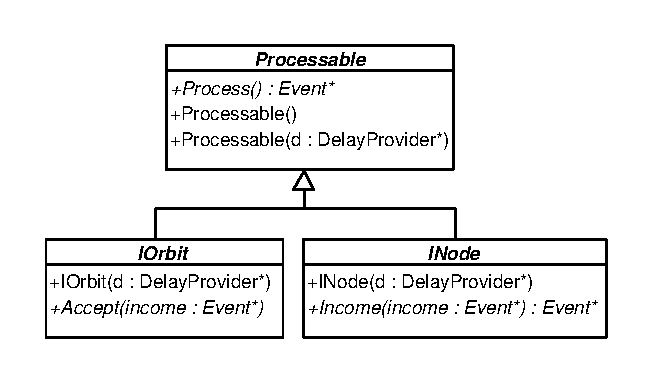
\includegraphics[scale=1]{inode_iorbit_uml.eps}
	\caption{Интерфейсы для обслуживающего прибора (INode) и орбиты (IOrbit), наследуемые от Processable}
	\label{inode_iorbit_uml}
\end{figure}
Метод IOrbit Accept служит для принятия заявок на орбиту, а метод INode Income - для принятия заявки на прибор для обслуживания. Отличие между данными методами заключается в том, что, если прибор занят обслуживанием другой заявки, то метод Income вернет заявку, которая пытается встать на прибор, в то время как орбита не имеет ограничения по количеству находящихся на ней заявок.

Для вычисления экспоненциальной задержки до наступления событий в модели, в предметную область был добавлен общий интерфейс для объектов, вычисляющих задержку, что позволяет менять способ вычисления задержки в процессе моделирования.
\begin{figure}[H]
	\centering
	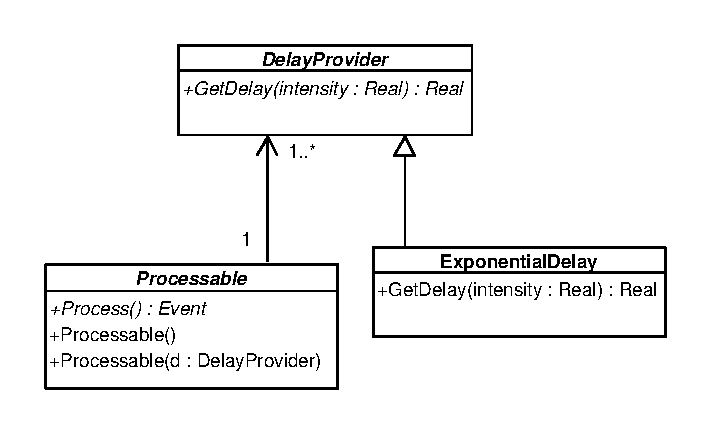
\includegraphics[scale=1]{delayprovider_uml.eps}
	\caption{DelayProvider - интерфейс для вычисления задержки, который используют элементы системы массового обслуживания}
	\label{delayprovider_uml}
\end{figure}

Для обеспечения среды, которой будет происходит моделирование, а именно - вестись подсчет прошедшего времени, взаимодействие с реализацией интерфейса Processable и сбор статистики, введен глобальный объект Environment
\begin{figure}[H]
	\centering
	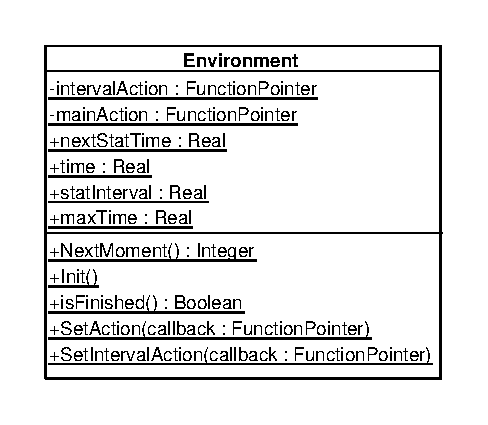
\includegraphics[scale=1]{environment_uml.eps}
	\caption{Глобальный объект Environment}
	\label{environment_uml}
\end{figure}

Статический класс Environment содержит общую для модели информацию - время моделирования, время конца моделирования и методы, для управления этими параметрами. 
Члены класса Environment будут описаны в последующих разделах.

\begin{figure}[H]
	\centering
	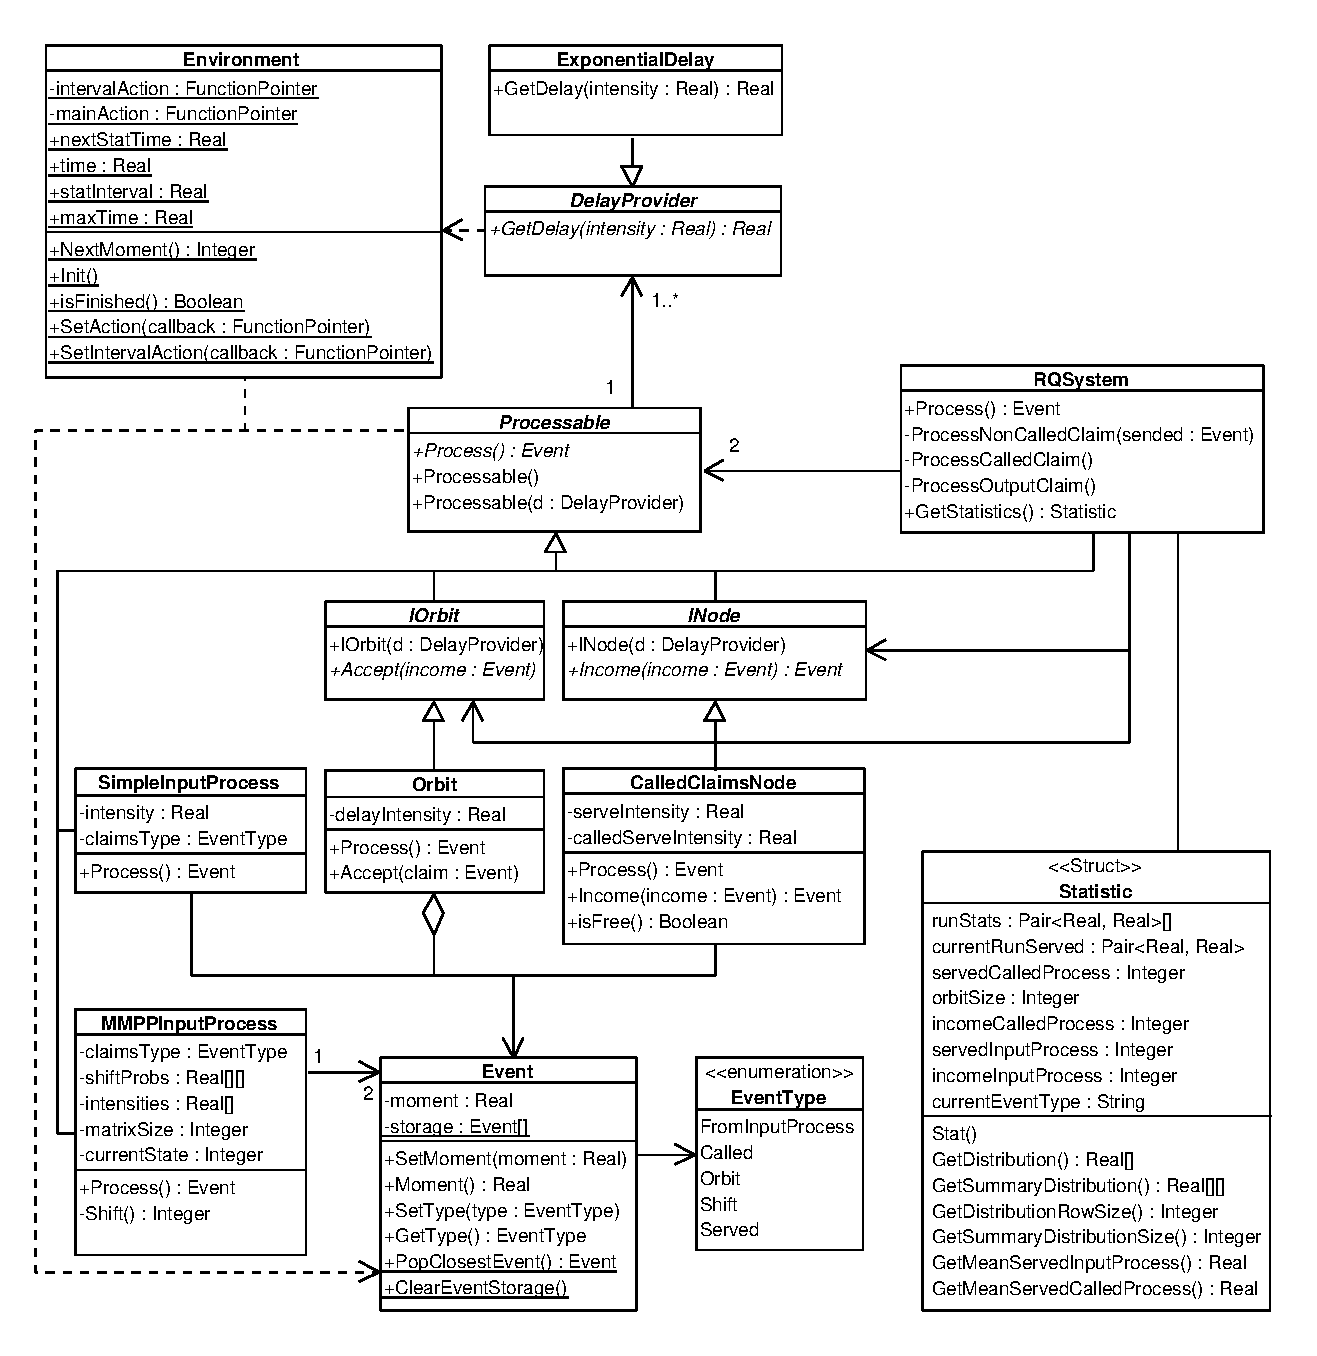
\includegraphics[scale=0.79]{domain_uml.eps}
	\caption{Предметная область имитационной модели}
	\label{domain_uml}
\end{figure}
На рисунке \ref{domain_uml} представлена полная предметная область программы. Определенные ранее интерфейсы реализуют конкретные элементы системы, используемые при моделировании. Поскольку, в данной работе рассматривается RQ-система с простейшим и MMPP-потоками, существует две соответствующих реализации входящего потока, подробности функционирования которых будут рассмотрены в следующем разделе. Таким образом, существуют следующие реализации элементов систем массового обслуживания:
\begin{itemize}
	\item Orbit - реализация источника повторных вызовов, содержащая хранилище заявок (Event), что на диаграмме классов показано агрегацией. Поле delayIntensity хранит интенсивность обращений заявок с орбиты, то есть используется для вычисления экспоненциальной задержки соответствующим объектом delayProvider.
	\item CalledClaimsNode - реализация обслуживающего прибора, способная обслуживать два типа заявок - пришедшие извне и вызванные, для чего служат интенсивности serveIntensity и calledServeIntensity соответственно.
	\item SimpleInputProcess - реализация простейшего входящего потока, порождающего заявки. Ассоциация с Event показывает, что класс имеет поле с заявкой, которая готовится покинуть источник заявок по истечении задержки.
	\item MMPPInputProcess - реализация MMPP-потока. Поле shiftProbs хранит матрицу интенсивностей переходов между состояниями, а поле intensities - интенсивность поступления заявок для каждого состояния. Логика смены состояний находится в приватном методе Shift, где используются поле currentState - номер текущего состояния, а так же объект Event, в котором хранится момент сменты состояния входящего потока, что на диаграмме показано ассоциацией с множителем.
	\item RQSystem представляет агрегирующий класс, где при помощи описанных выше классов строится логика работы системы.
\end{itemize}
\clearpage
\subsection{Процесс моделирования}
В качестве среды для моделирования в реализованной программе выступает глобальный объект Environment, представленный на рисунке \ref{environment_uml}.В процессе моделирования у Environment вызывается метод NextMoment, который переносит систему в следующий момент моделирования, то есть, совершается одна итерация процесса моделирования. Перед началом моделирования вызывается метод Init, который подготавливает модель к началу работы. Метод isFinished служит для осведомления других участков программы, что моделирование окончено, то есть, что выставленное время моделирования (maxTime) прошло.

Для обеспечения гибкости действий, которые модель может совершать в процессе работы, метод NextMoment имеет частичную реализацую, в которой вызывается указатель на функцию или лямбда-выражение mainAction. Таким образом, поведение модели можно менять в процессе ее работы, что делает класс Environment универсальным для многих систем, использующих пошаговое моделирование.
\begin{figure}[H]
	\centering
	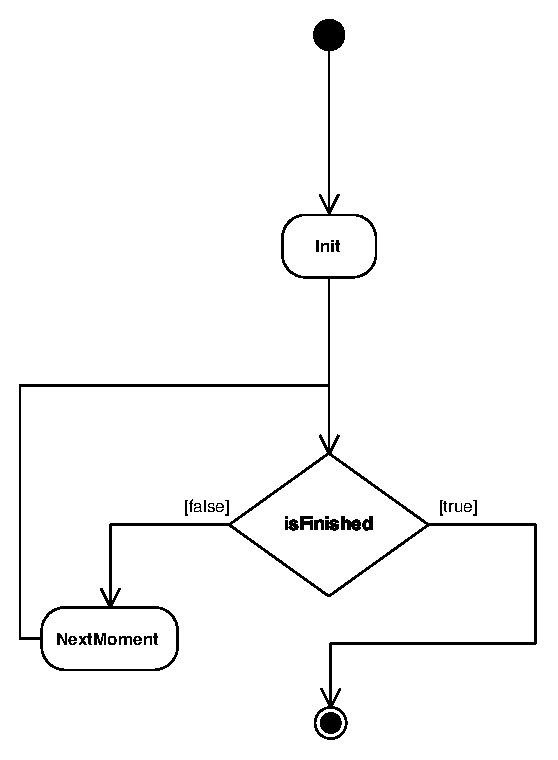
\includegraphics[scale=0.8]{simulation_algo_uml.eps}
	\caption{Общий алгоритм процесса моделирования на основе класса Environment}
	\label{simulation_algo_uml}
\end{figure}

Для сбора статистики и построения распределения количества обслуженных заявок, в классе Environment предусмотрен механизм интервального сбора данных моделирования. Поле statInterval хранит интервал модельного времени, по прошествии которого должен производится вызов функции или лямбда выражения по указателю intervalAction, в котором задается логика сбора данных.
\begin{figure}[H]
	\centering
	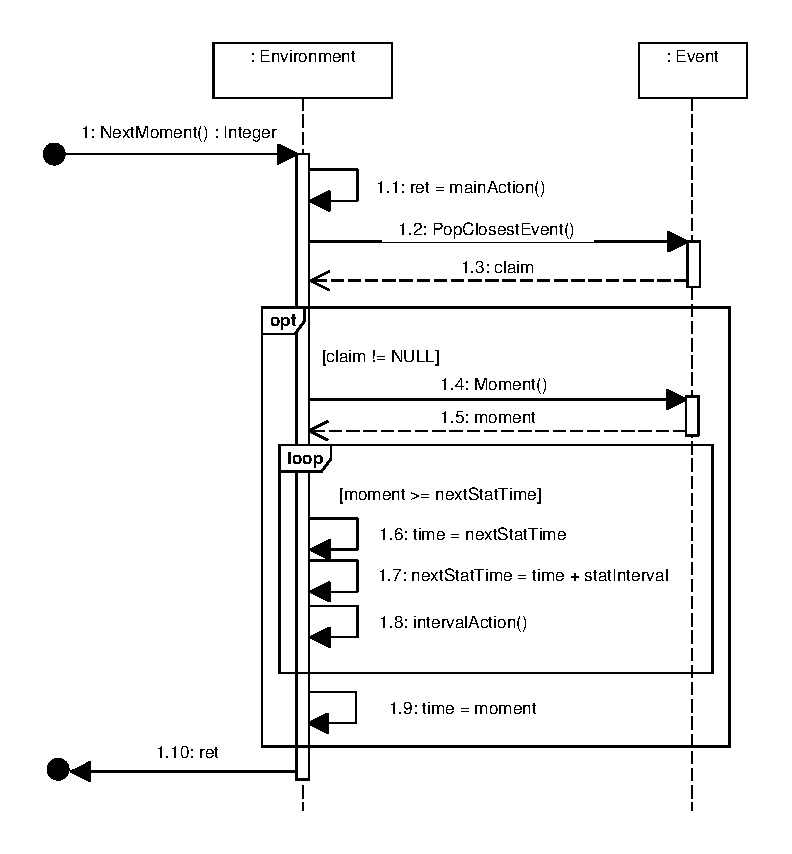
\includegraphics[scale=0.8]{next_moment_algo_uml.eps}
	\caption{Алгоритм метода NextMoment}
	\label{next_moment_algo_uml}
\end{figure}
Функционирование же отдельным элементов системе описывается в методах интерфейса Processable и наследуемых от него INode и IOrbit.
Происходящее с обслуживающим прибором во время очередной итерации отражено на диаграммах последовательностей \ref{CalledClaimsNode_Process_uml} и \ref{}
\begin{figure}[H]
	\centering
	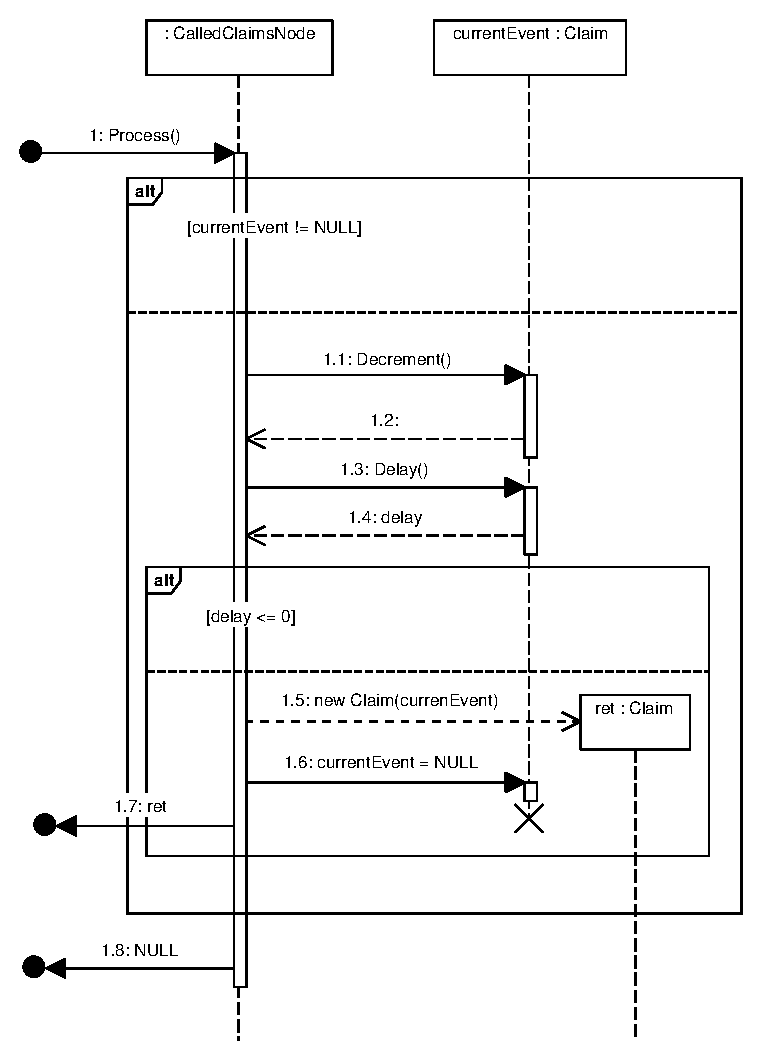
\includegraphics[scale=0.9]{CalledClaimsNode_Process.eps}
	\caption{Диаграмма последовательностей метода Process класс CalledClaimsNode}
	\label{CalledClaimsNode_Process_uml}
\end{figure}
Если прибор на данный момент не обслуживает заявку currentEvent (поле currentEvent на диаграмме \ref{domain_uml} обозначено ассоциацией), то возвращается NULL, говорящий о том, что на данной итерации прибор не закончил обслуживание заявки, так как он либо свободен, либо обслуживание еще в процессе. Иначе, задержка то конца обслуживания заявки на приборе уменьшается вызовом метода Decrement(). За этим, производится проверка, вышло ли время обслуживания заявки. В случае, если вышло, обслуженная заявка возращается, а прибор становится свободным.
\begin{figure}[H]
	\centering
	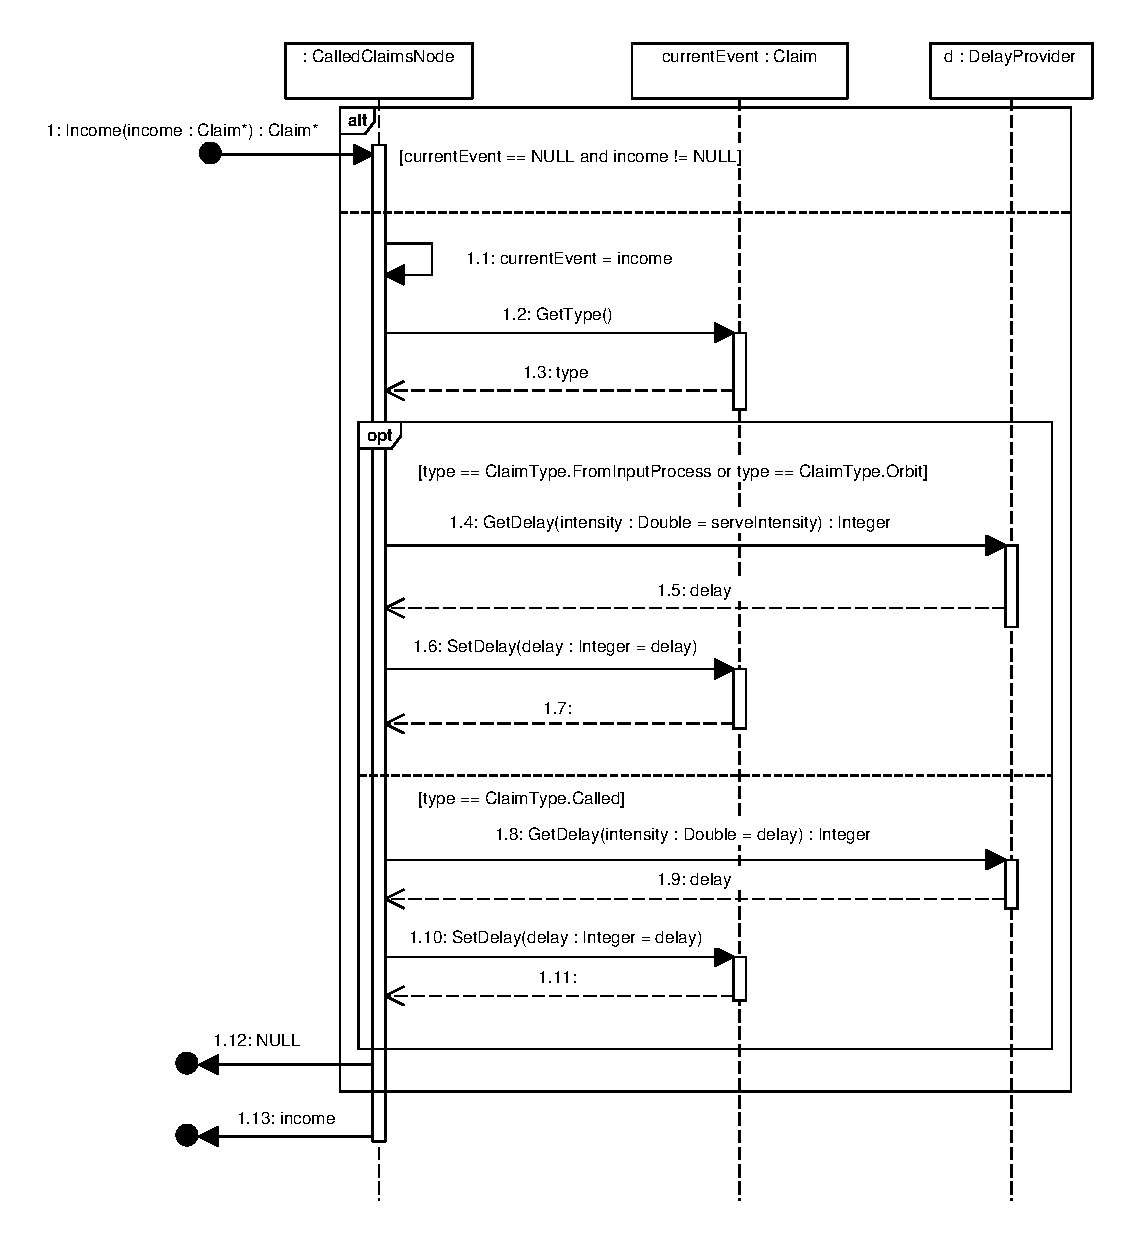
\includegraphics[scale=0.9]{CalledClaimsNode_Income.eps}
	\caption{Диаграмма последовательностей метода Income класс CalledClaimsNode}
	\label{CalledClaimsNode_Income_uml}
\end{figure}